\subsection{Color Swap}
The button to swap colours had no functionality other than swapping the colour on the preview button itself, thus the swap would not affected other parts of the program.
To resolve this issue, the class diagram was used to identify a connection between the preview button and the draw view.
As seen in \figref{fig:clsdiagramsnippet}, two connections are found between \textit{DravView} and \textbf{PreviewButton}, which is \textit{ColorButton} and \textit{DrawFragment}.
\textit{ColorButton} is used when picking a new colour, and assigns this new colour to \textit{PreviewButton}.
However, when pressing the \textit{PreviewButton}, no connection existed.
In order to correct this issue, the event for touching \textit{PreviewButton} could be accessed from \textit{DrawFragment} and was already implemented for the other buttons. 
\fxwarning{Har fjernet denne figur da den giver problemer}
%\begin{figure}
%     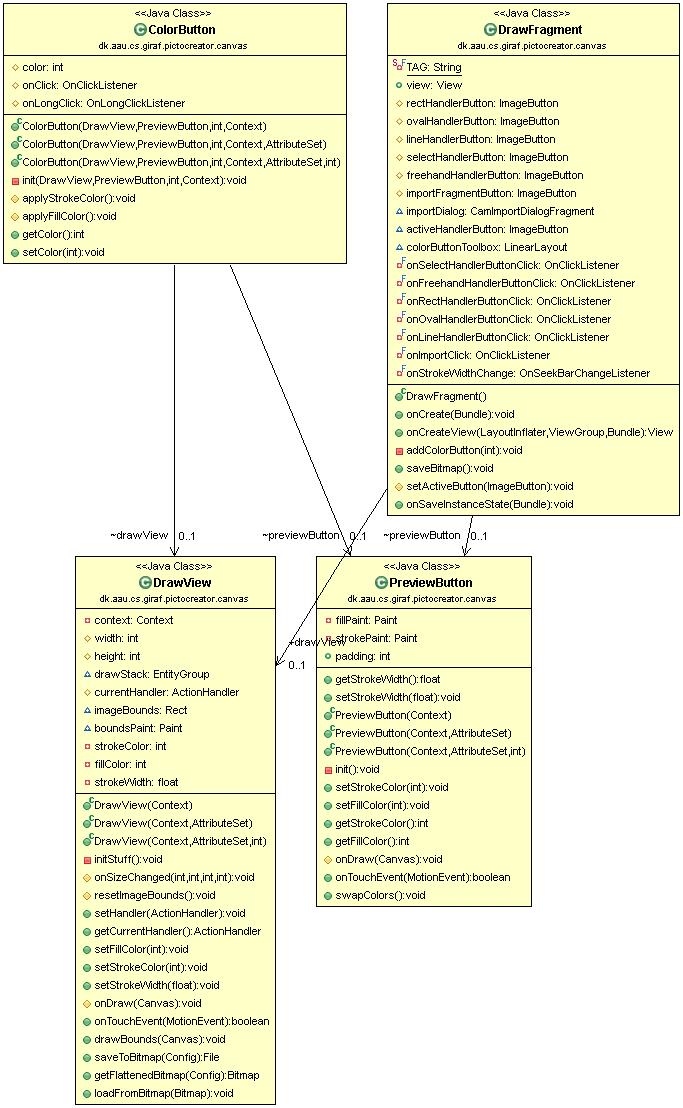
\includegraphics[scale=0.5]{media/classdiagram-swapcolour-issue.gif}
%     \caption{Snippet of class diagram.}\label{fig:clsdiagramsnippet}
%\end{figure}

In order to correct this issue, the \textit{onTouch} event was moved from \textit{PreviewButton} to \textit{DrawFragment}, since \textit{DrawFragment} had access to both \textit{DrawView} and \textit{PreviewButton}.
\textit{DrawFragment} was already subscribed to the other buttons, thus it was a logical change to move the touch event of \textit{PreviewButton} to \textit{DrawFragment}.
The event implemented in \textit{DrawFragment} can be seen in \lstref{event-previewbuttonclick}.

\begin{lstlisting}[caption={onPreviewButtonClick event},label=lst:event-previewbuttonclick]
private final OnClickListener onPreviewButtonClick = new OnClickListener() {
    @Override
    public void onClick(View v) {
       previewButton.swapColors();
       drawView.setFillColor(previewButton.getFillColor());
       drawView.setStrokeColor(previewButton.getStrokeColor());
    }
};
\end{lstlisting}